\documentclass[tikz,margin=2mm]{standalone}

\usetikzlibrary{matrix}
\tikzset{
    sup/.style={label={[minimum size=0,font=\scriptsize,anchor=north west,shift={(-10mm-0.5\pgflinewidth,-1.5mm)}]#1}},
    sub/.style={label={[minimum size=0,font=\tiny,anchor=north west,shift={(-10mm-0.5\pgflinewidth,-12mm)}]#1}},
    co1/.style={fill=blue!50},
    co2/.style={fill=green!50},
    co3/.style={fill=yellow!50},
    co4/.style={fill=purple!50},
    co5/.style={fill=orange!50},
    co6/.style={fill=red!50},
    my empty cell/.style={minimum size=2cm,fill=none,draw=none},
    table of arguments/.style={
        matrix of nodes,
        column sep=-\pgflinewidth,
        row sep=-\pgflinewidth,
        inner sep=1mm,
        nodes={
            minimum size=2cm,
            draw,
            anchor=center,
            fill,
            text width=1.8cm,
            font=\ttfamily\LARGE,
            align=justify,
        },
    },
    alpha quadrant/.style={
        table of arguments,
        name=alpha,
        matrix anchor=south west,
        co1/.append style={sup={1 Pre FF}},
        co2/.append style={sup={1 Pre VF}},
        co3/.append style={sup={1 Pre VV}},
        co4/.append style={sup={1 Pre PF}},
        co5/.append style={sup={1 Pre PV}},
    },
    beta quadrant/.style={
        table of arguments,
        name=beta,
        matrix anchor=south east,
        co1/.append style={sup={1 Sub FF}},
        co3/.append style={sup={1 Sub VV}},
        co4/.append style={sup={1 Sub PF}},
        co6/.append style={sup={1 Sub PP}},
    },
    gamma quadrant/.style={
        table of arguments,
        name=gamma,
        matrix anchor=north east,
        co2/.append style={sup={2 Sub VF}},
        co3/.append style={sup={2 Sub VV}},
        co4/.append style={sup={2 Sub PF}},
    },
    delta quadrant/.style={
        table of arguments,
        name=delta,
        matrix anchor=north west,
        co2/.append style={sup={2 pre VF}},
        co3/.append style={sup={2 pre VV}},
        co4/.append style={sup={2 pre PF}},
        co5/.append style={sup={2 pre PV}},
        co6/.append style={sup={2 pre PP}},
    },
}

\begin{document}
    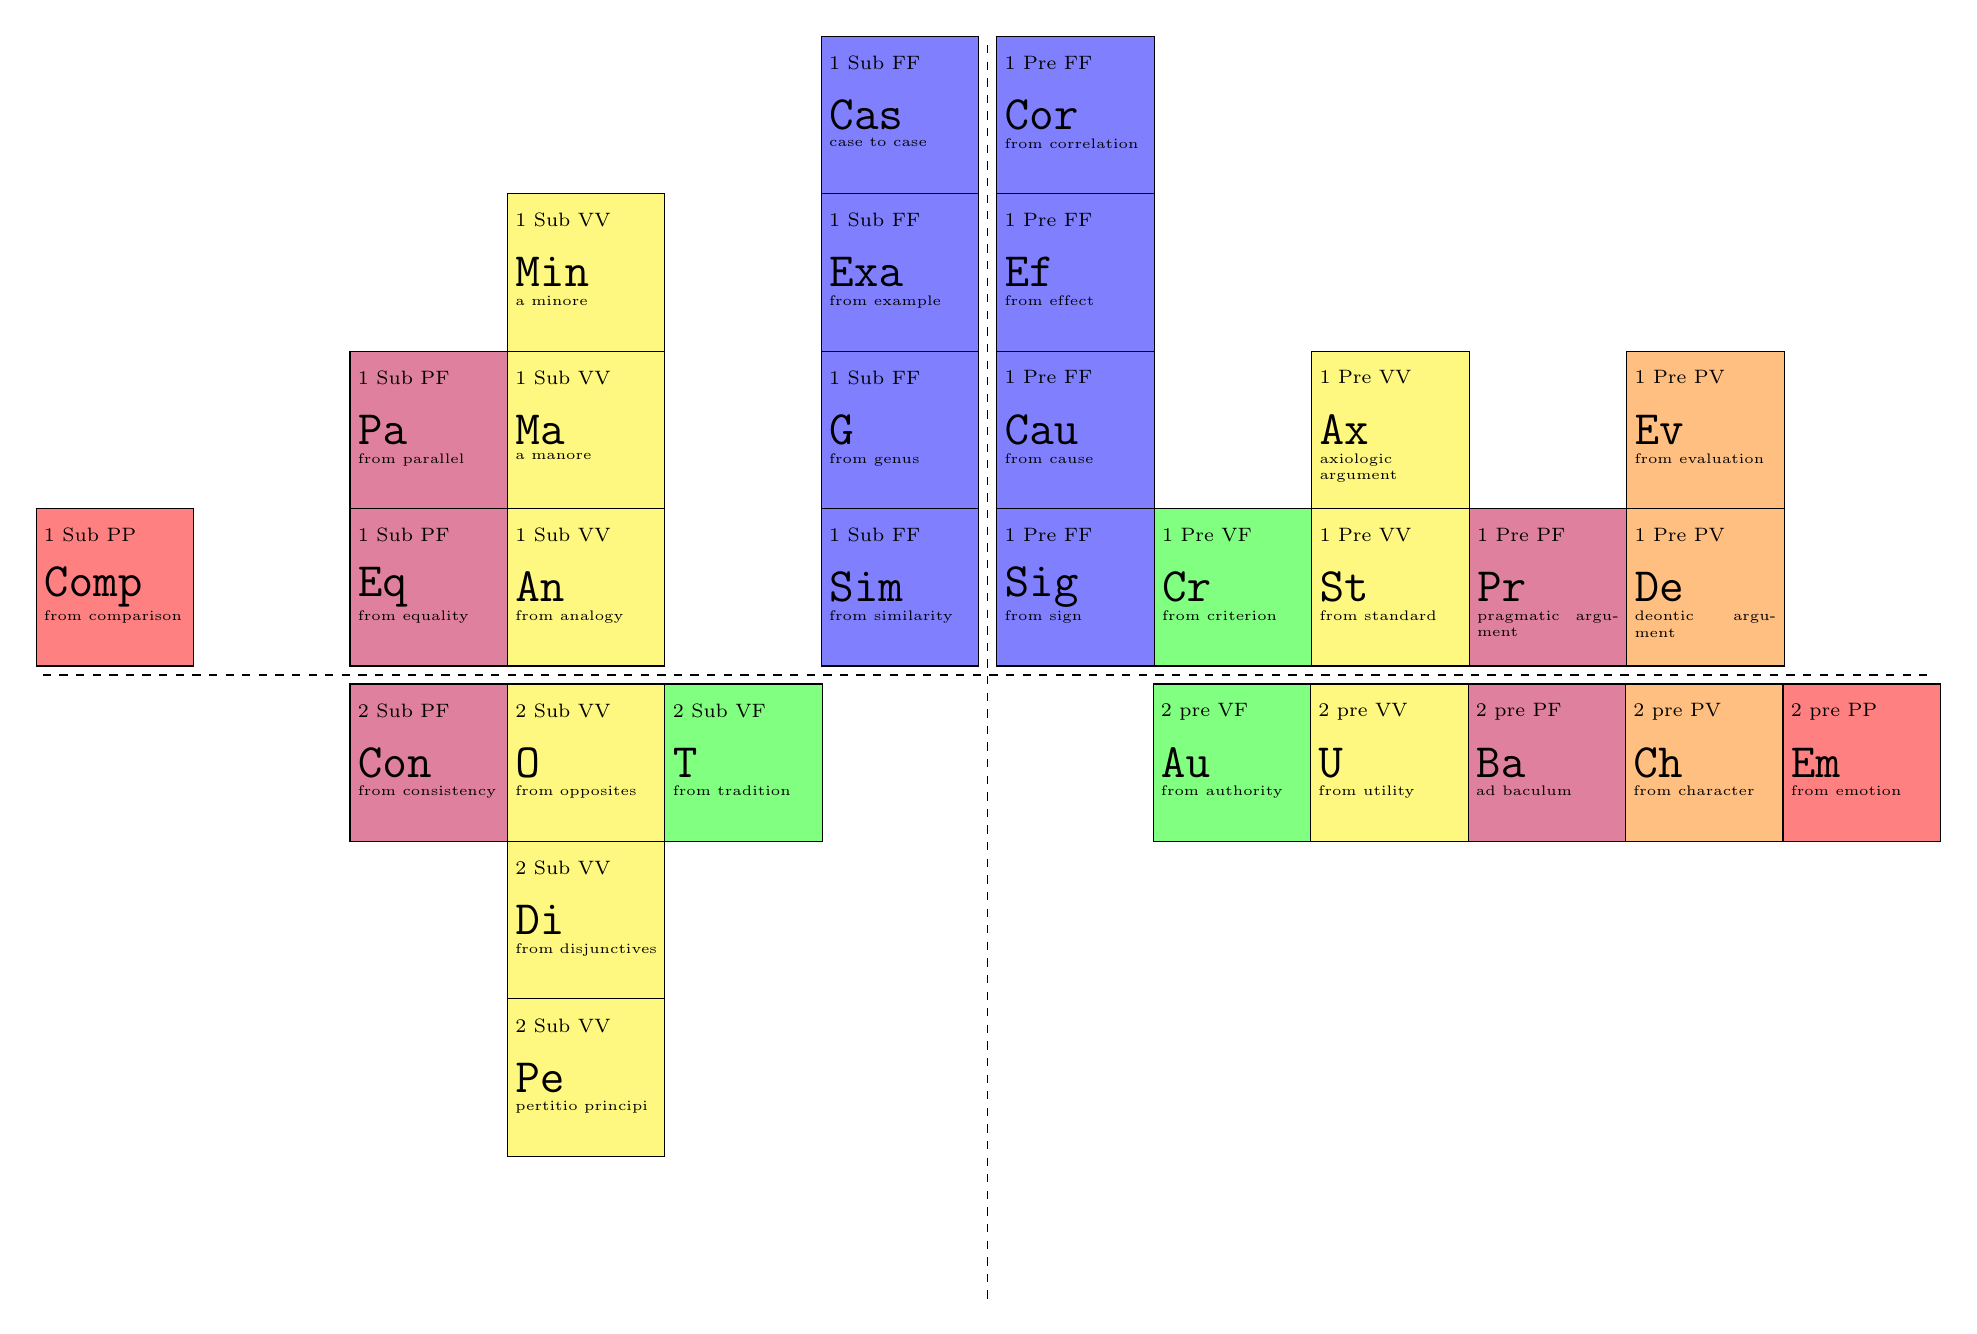
\begin{tikzpicture}
        \matrix[alpha quadrant]{
            |[co1,sub={from correlation}]|Cor &                                 &                                     &                                     &                                   & \\
            |[co1,sub={from effect}]| Ef      &                                 &                                     &                                     &                                   & \\
            |[co1,sub={from cause}]| Cau      &                                 & |[co3,sub={axiologic argument}]| Ax &                                     & |[co5,sub={from evaluation}]| Ev  & \\
            |[co1,sub={from sign}]| Sig       & |[co2,sub={from criterion}]| Cr & |[co3,sub={from standard}]| St      & |[co4,sub={pragmatic argument}]| Pr & |[co5,sub={deontic argument}]| De & \\
        };
        \matrix[beta quadrant]{
                                               &                   &                                &                               &                   & |[co1,sub={case to case}]| Cas \\
                                               &                   &                                & |[co3,sub={a minore}]| Min    &                   & |[co1,sub={from example}]| Exa\\
                                               &                   & |[co4,sub={from parallel}]| Pa & |[co3,sub={a manore}]| Ma     &                   & |[co1,sub={from genus}]| G \\
            |[co6,sub={from comparison}]| Comp & |[my empty cell]| & |[co4,sub={from equality}]| Eq & |[co3,sub={from analogy}]| An & |[my empty cell]| & |[co1,sub={from similarity}]| Sim \\
        };
        \matrix[gamma quadrant]{
            |[co4,sub={from consistency}]| Con & |[co3,sub={from opposites}]| O     & |[co2,sub={from tradition}]| T & |[my empty cell]| \\
                                               & |[co3,sub={from disjunctives}]| Di &                                &                   \\
                                               & |[co3,sub={pertitio principi}]| Pe &                                &                   \\
        };
        \matrix[delta quadrant]{
            |[my empty cell]| & |[co2,sub={from authority}]| Au & |[co3,sub={from utility}]| U & |[co4,sub={ad baculum}]| Ba & |[co5,sub={from character}]| Ch & |[co6,sub={from emotion}]| Em \\
        };
        \draw[dashed] (0,8) -- (0,-8)
            (-12,0) -- (12,0);
    \end{tikzpicture}
\end{document}
